		\chapter{Analysis and Design}
		\section{Methodology / Procedure adopted}
		\begin{itemize}
		\item The common ways adopted by people for plagiarizing the code are:
		\begin{enumerate}
		 \item The original source code can be replicated as it is.
		 \item Addition of comments in the source code.
		 \item Modification in identifiers. 
		 \item Chane in variable position.
		 \item The procedure combination can be done in source code.
		 \item Program statements can be changed by some modifications.
		 \item Control Logic can be modified.
		 \end{enumerate}
		\item Describe on the development methodology / model you would use. (E.g. Agile method or Iterative Model)
		\begin{enumerate}
		\item In Iterative model, iterative process starts with a simple implementation of a small set of the software requirements and iteratively enhances the evolving versions until the complete system is implemented and ready to be deployed.
		\item An iterative life cycle model does not attempt to start with a full specification of requirements. Instead, development begins by specifying and implementing just part of the software, which is then reviewed in order to identify further requirements. This process is then repeated, producing a new version of the software at the end of each iteration of the model.\\
		\end{enumerate}
		\item How you intend manage the weekly meetings ? \\
		The weekly meetings need to managed properly because in order to accomplish the goals desired, you will need to have a good strategic and tactical plan. In the meeting, plans may be decided by each team member and the procedure is been planned.
		\item How do you intend to monitor and measure the progress of the project? \\ 
		The monitoring and measure of progress of report is been done on basis of different modules. A schedule is maintained for each module to be complemented. Github is used for project monitoring ,as all the team members upload their work on completion. 
		\end{itemize}
		\section{Analysis}
		
		Based on the requirements gathered, how was the feasibility study of the project carried out? \\
		The project is about the detection of software source code plagiarism, so the study carried out on the comparison of the different plagiarism software's which are based on rule based algorithms.\\
		On comparison of different features of some software's.\\
		The papers were referred for plagiarism detection, which gives the idea of different levels of plagiarism and defining the metrics for the programs.  \\
		If any requirements, were modified why they were modified? \\
		
		
		\section{Proposed System}
		
		Committing plagiarism is extremely easy as we can simply copy paste code and claim it as our own. There are lots of techniques like changing variable names, adding comments, changing the loop types which are used to hide the plagiarism. For this reason, sophisticated plagiarism detection software is needed to prevent plagiarism in both educational institutions and software industry. 
		
		Therefore, we propose this system that can detect different kinds of plagiarism. 
		
		\subsection{Hardware / Software requirements}
		\begin{itemize}
		
		
		\item Development Hardware / Software requirements \\\\
		Software Requirements : \\
		Java  JDK 1.4 or more \\
		Operating System : Window/Linux\\
		Front-End : Java Fx\\
		Back-End : MySQL\\\\
		Hardware Requirements :\\
		Minimum Memory : 512 Mb RAM \\
		Hard disk space : 1 GB\\\\
		
		
		\item Deployment Hardware / Software requirements \\\\
		Software Requirements : \\
		Java Runtime Environment\\
		Operating System : Window/Linux. \\\\
		Hardware Requirements : \\
		Minimum Memory : 512 Mb RAM \\
		Hard disk space : 1 GB\\
		\end{itemize}
		\subsection{Design Details}
		  \begin{itemize}
		  
		  \item Data Flow Diagram Level 0\\
		  
		  
		  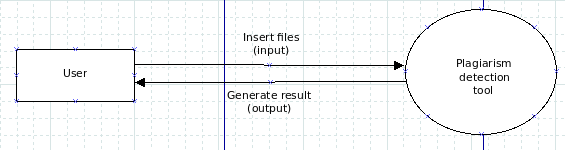
\includegraphics[width=1\textwidth]{DFD_lvl0}
		  
		  \label{fig:DFD_Level0}
		  
		  
		  
			\item Data Flow Diagram Level 1\\  
		  
		   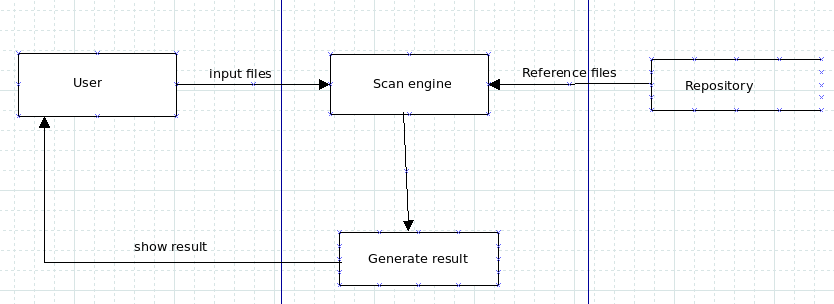
\includegraphics[width=1\textwidth]{DFD_lvl1}
		   
		  \label{fig:DFD_Level1}
		  
		  
			\item Flowchart\\
		  
		   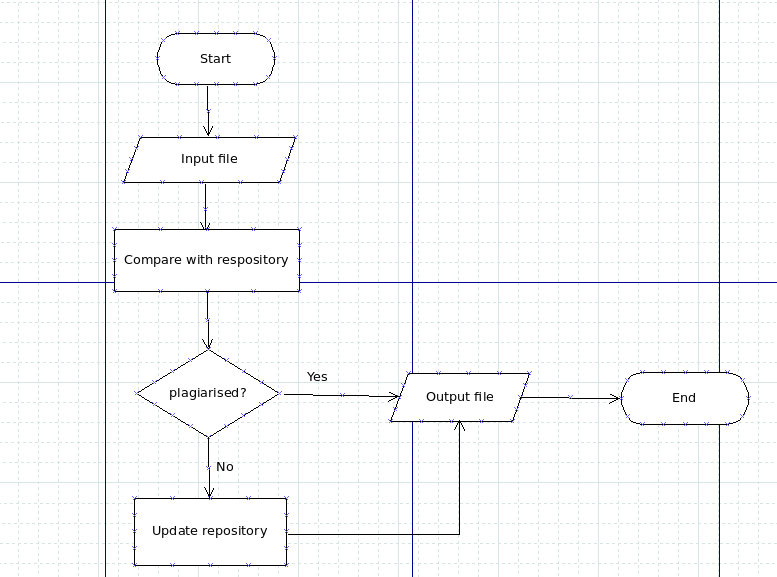
\includegraphics[width=1\textwidth]{Flowchart}
		   
		  \label{fig:Flowchart}
		  
		  \item Use Case Diagram\\
		  
		  
		   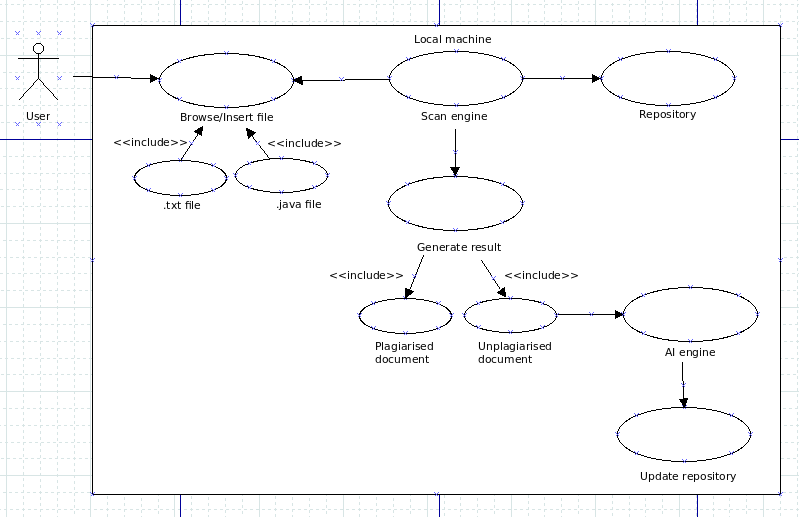
\includegraphics[width=1\textwidth]{UseCaseDiag}
		   
		  \label{fig:Use_Case_Diagram}
				
				
		
		  \end{itemize}		
		
		
		
		
				
		\subsection{Implementation Plan}
		
		  
		  
		  
		  
		  Timeline chart is as follows
	
		   \begin{figure}
		   	  \centering
		   \hfill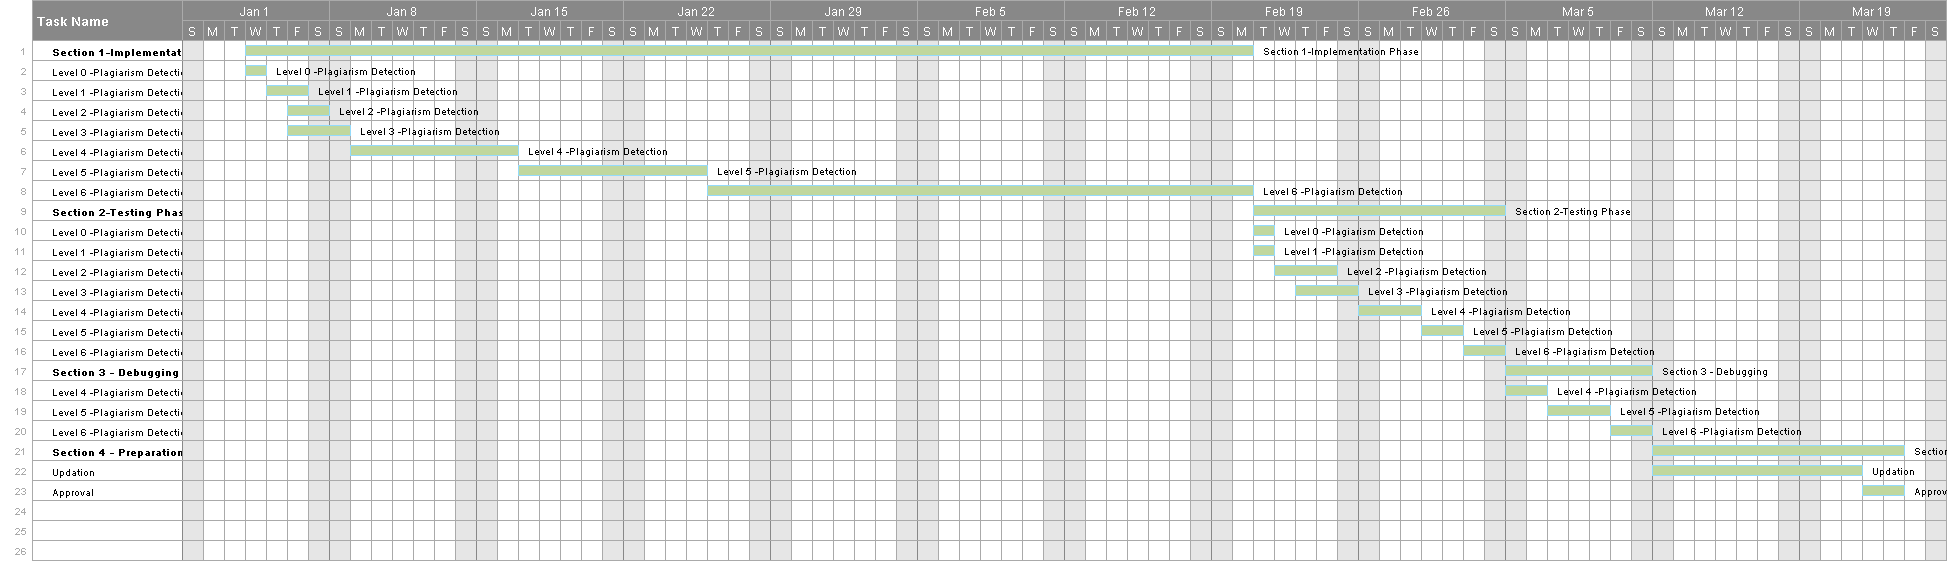
\includegraphics[scale=.380,angle=90]{Timeline}\hspace{\fill}
		   \caption{Timeline chart}
		   \end{figure}
				
				
		
		  	
		
		
		
		
		
		
		
		
		
